この節では変数、定数、Goの内部クラスの定義と、Goプログラムの設計におけるテクニックをご紹介します。

\subsubsection{変数の定義}
Go言語では変数は数多くの方法で定義されます。

\texttt{var}キーワードを使用することはGoの最も基本的な変数の定義方法です。C言語と異なり、Goでは変数の型を変数の後に置きます。


\begin{lstlisting}[numbers=none]
//"variableName"という名前で定義します。型は"type"です。
var variableName type
\end{lstlisting}

複数の変数を定義します。

\begin{lstlisting}[numbers=none]
//すべて"type"型の3つの変数を定義します。
var vname1, vname2, vname3 type
\end{lstlisting}

変数を定義し、初期化します。

\begin{lstlisting}[numbers=none]
//"variableName"の変数を"value"で初期化します。型は"type"です。
var variableName type = value
\end{lstlisting}

複数の変数を同時に初期化します。

\begin{lstlisting}[numbers=none]
/*
  すべてが"type"型となる変数をそれぞれ定義し、個別に初期化を行います。
  vname1はv1,vname2はv2,vname3はv3
*/
var vname1, vname2, vname3 type= v1, v2, v3
\end{lstlisting}

あなたは上述の定義が面倒だと思いますか?大丈夫、Go言語の設計者もわかっています。少し簡単に書くこともできます。直接型の宣言を無視することができるので、上のコードはこのようにも書けます:

\begin{lstlisting}[numbers=none]
/*
   3つの変数を定義し、それぞれ個別に初期化する。
   vname1はv1,vname2はv2,vname3はv3
   このあとGoは代入される値の肩に従ってそれぞれ初期化を行います。
*/
var vname1, vname2, vname3 = v1, v2, v3
\end{lstlisting}

これでもまだ面倒ですか?ええ、私もそう思います。更に簡単にしてみましょう。

\begin{lstlisting}[numbers=none]
/*
   3つの変数を定義し、それぞれ個別に初期化します。
   vname1はv1,vname2はv2,vname3はv3
   コンパイラは初期化する値に従って自動的にふさわしい型を導き出します。
*/
vname1, vname2, vname3 := v1, v2, v3
\end{lstlisting}

これなら非常に簡潔になったでしょう?\texttt{:=}の記号は\texttt{var}と\texttt{type}に直接取って代わるものです。これらの形式を短縮宣言と呼びます。ただしこれにはひとつ制限があります。これらは関数の内部でしか使用できません。関数の外で使用するとコンパイルが通らなくなります。そのため、一般的には\texttt{var}方式でグローバル変数が定義されます。

\texttt{\_}(アンダースコア)は特別な変数名です。どのような値もすべて捨てられてしまいます。この例では\texttt{35}という値を\texttt{b}に与えますが、同時に\texttt{34}は失われてしまいます。

\begin{lstlisting}[numbers=none]
_, b := 34, 35
\end{lstlisting}

Goはすでに宣言されている未使用の変数をコンパイル時にエラーとして出力します。例えば下のコードはエラーを一つ生成します。\texttt{i}は宣言されましたが使用されていません。

\begin{lstlisting}[numbers=none]
package main

func main() {
    var i int
}
\end{lstlisting}





\subsubsection{定数}
いわゆる定数というのは、プログラムがコンパイルされる段階で値が決定されます。そのため、プログラムが実行される時には値の変更は許されません。定数には数値、bool値または文字列等の型を定義することができます。

この文法は以下の通りです:

\begin{lstlisting}[numbers=none]
const constantName = value
//もし必要であれば、定数の型を明示することもできます:
const Pi float32 = 3.1415926
\end{lstlisting}

ここでは定数の宣言の例を示します:

\begin{lstlisting}[numbers=none]
const Pi = 3.1415926
const i = 10000
const MaxThread = 10
const prefix = "astaxie_"
\end{lstlisting}

Go の定数は一般的なプログラミング言語と異なり、かなり多くの小数点以下の桁を指定することができます(たとえば200桁など)、 float32に自動的な32bitへの短縮を指定したり、float64に自動的な64bitへの短縮を指定するにはリンク(http:\//\//golang.org\//ref\//spec\#Constants)をご参照ください。

\subsubsection{ビルトイン基本型}
\paragraph{Boolean}
Goではbool値の型は\texttt{bool}です。値は\texttt{true}もしくは\texttt{false}です。デフォルト値は\texttt{false}です。

\begin{lstlisting}[numbers=none]
// コード例
var isActive bool  // グローバル変数の宣言
var enabled, disabled = true, false  // 型を省略した宣言
func test() {
    var available bool  // 通常の宣言
    valid := false      // 短縮宣言
    available = true    // 代入操作
}
\end{lstlisting}

\paragraph{数値型}
整数型には符号付きと符号無しの2つがあります。Goはまた\texttt{int}と\texttt{uint}をサポートしています。この2つの型の長さは同じですが、実際の長さは異なるコンパイラによって決定されます。Goでは直接bit数を指定できる型もあります:\texttt{rune}, \texttt{int8}, \texttt{int16}, \texttt{int32}, \texttt{int64}と\texttt{byte}, \texttt{uint8}, \texttt{uint16}, \texttt{uint32}, \texttt{uint64}です。この中で\texttt{rune}は\texttt{int32}のエイリアスです。\texttt{byte}は\texttt{uint8}のエイリアスです。

\begin{quote}
注意しなければならないのは、これらの型の変数間は相互に代入または操作を行うことができないということです。コンパイル時にコンパイラはエラーを発生させます。

下のコードはエラーが発生します。:invalid operation: a + b (mismatched types int8 and int32)
\begin{lstlisting}[numbers=none]
    var a int8
    var b int32
    c:=a + b
\end{lstlisting}
また、intの長さは32bitですが、intとint32もお互いに利用することはできません。
\end{quote}

浮動小数点の型には\texttt{float32}と\texttt{float64}の二種類があります(\texttt{float}型はありません。)。デフォルトは\texttt{float64}です。

これで全てですか?No! Goは複素数もサポートしています。このデフォルト型は\texttt{complex128}(64bit実数+64bit虚数)です。もしもう少し小さいのが必要であれば、\texttt{complex64}(32bit実数+32bit虚数)もあります。複素数の形式は\texttt{RE + IMi}です。この中で\texttt{RE}が実数部分、\texttt{IM}が虚数部分になります。最後の\texttt{i}は虚数単位です。以下に複素数の使用例を示します:

\begin{lstlisting}[numbers=none]
var c complex64 = 5+5i
//output: (5+5i)
fmt.Printf("Value is: %v", c)
\end{lstlisting}

\paragraph{文字列}
前の章で述べた通り、Goの文字列はすべて\texttt{UTF-8}コードが採用されています。文字列は一対のダブルクォーテーション(\texttt{""})またはバッククォート(\texttt{` `} )で括られることで定義されます。この型は\texttt{string}です。

\begin{lstlisting}[numbers=none]
//コード例
var frenchHello string  // 文字列変数の宣言の一般的な方法
var emptyString string = ""
// 文字列変数を一つ宣言し、空文字列で初期化する。
func test() {
    no, yes, maybe := "no", "yes", "maybe"
    // 短縮宣言、同時に複数の変数を宣言
    japaneseHello := "Konichiwa"  // 同上
    frenchHello = "Bonjour"  // 通常の代入
}
\end{lstlisting}

Goの文字列は変更することができません。例えば下のコードはコンパイル時にエラーが発生します。:cannot assign to s[0]

\begin{lstlisting}[numbers=none]
var s string = "hello"
s[0] = 'c'
\end{lstlisting}

ただし、本当に変更したくなったらどうしましょうか?ここでは以下のコードで実現します:

\begin{lstlisting}[numbers=none]
s := "hello"
c := []byte(s)  // 文字列 s を []byte 型にキャスト
c[0] = 'c'
s2 := string(c)  // もう一度 string 型にキャストし直す
fmt.Printf("%s\n", s2)
\end{lstlisting}

Goでは+演算子を使って文字列を連結することができます:

\begin{lstlisting}[numbers=none]
s := "hello,"
m := " world"
a := s + m
fmt.Printf("%s\n", a)
\end{lstlisting}

文字列の修正もこのように書けます:

\begin{lstlisting}[numbers=none]
s := "hello"
s = "c" + s[1:] // 文字列を変更することはできませんが
                // スライスは行えます。
fmt.Printf("%s\n", s)
\end{lstlisting}

もし複数行の文字列を宣言したくなったらどうしましょうか?この場合\texttt{` }で宣言することができます:

\begin{lstlisting}[numbers=none]
m := `hello
    world`
\end{lstlisting}

\texttt{`} で括られた文字列はRaw文字列です。すなわち、文字列はコード内の形式がそのままプリント時の形式になります。文字列の変更はありません。改行はそのまま出力されます。例えばこの例では以下のように出力されます:

\begin{lstlisting}[numbers=none]
hello
    world
\end{lstlisting}


\paragraph{エラー型}
Goにはビルトインの\texttt{error}型があります。専らエラー情報の処理に使用されます。Goの\texttt{package}の中にはエラー処理を行う\texttt{errors}というパッケージがあります。


\begin{lstlisting}[numbers=none]
err := errors.New("emit macho dwarf: elf header corrupted")
if err != nil {
    fmt.Print(err)
}
\end{lstlisting}

\subsubsection{Goデータの低レイヤの保存}
下の図はRuss Cox Blogの中の一文で紹介されているGoデータ構造の文章です。これらの基本型は低レイヤでメモリを分配し、対応する値を保存していることが見て取れるとおもいます。

\begin{figure}[H]
  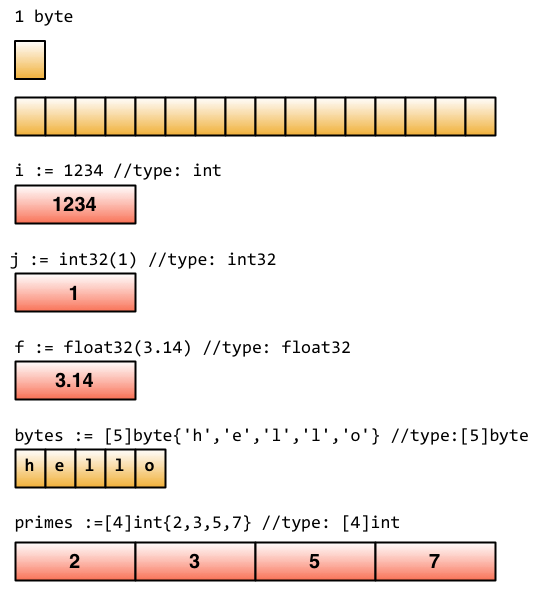
\includegraphics[width=14cm]{2.2.basic.png}
   \label{図2.1}
   \caption{Goデータ形式の保存}
\end{figure}

\subsubsection{テクニック}
\paragraph{グループ化による宣言}
Go言語では、複数の定数・変数を宣言する場合、または複数のパッケージをインポートする場合、グループ化による方法で宣言することができます。

例えば以下のコード:

\begin{lstlisting}[numbers=none]
import "fmt"
import "os"

const i = 100
const pi = 3.1415
const prefix = "Go_"

var i int
var pi float32
var prefix string
\end{lstlisting}

グループ化によって以下のような形式になります:

\begin{lstlisting}[numbers=none]
import(
    "fmt"
    "os"
)

const(
    i = 100
    pi = 3.1415
    prefix = "Go_"
)

var(
    i int
    pi float32
    prefix string
)
\end{lstlisting}



\paragraph{iota列挙型}
Goでは\texttt{iota}というキーワードがあります。このキーワードは\texttt{enum}を宣言する際に使用されます。このデフォルト値は0からはじまり、順次1が追加されます:



\begin{lstlisting}[numbers=none]
const(
    x = iota  // x == 0
    y = iota  // y == 1
    z = iota  // z == 2
    w  // 定数の宣言で値を省略した場合、デフォルト値は
       // 前の値と同じになります。ここではw = iotaと
       // 宣言していることと同じになりますので、
       // w == 3となります。実は上のyとzでも
       // この"= iota"は省略することができます。
)

 const v = iota // constキーワードが出現する度に、
          // iotaは置き直されます。ここではv == 0です。

const ( 
  e, f, g = iota, iota, iota //e=0,f=0,g=0 iotaの同一行は同じです
  )
\end{lstlisting}

\begin{quote}
他の値や\texttt{iota}に設定されているものを除いて、各\texttt{const}グループのはじめの定数はデフォルトで0となります。二番目以降の定数は前の定数の値がデフォルト値となります。もし前の定数の値が\texttt{iota}であれば、直後の値も\texttt{iota}になります。
\end{quote}


\subsubsection{Goプログラムのデザインルール}
Goがこのように簡潔なのは、それがいくつかのデフォルトの行為を持っているからです:

\begin{itemize}
  \item 大文字で始まる変数はエクスポート可能です。つまり、他のパッケージから読むことができる、パブリックな変数だということです。対して小文字で始まる変数はエクスポートできません。これはプライベート変数です。
  \item 大文字で始まる関数も同じです。\texttt{class}の中で\texttt{public}キーワードによってパブリック関数となっているのと同じです。対して小文字で始まる関数は\texttt{private}キーワードのプライベート関数です。
\end{itemize}

\paragraph{array}
\texttt{array}は配列です。この定義は以下のようになります:

\begin{lstlisting}[numbers=none]
var arr [n]type
\end{lstlisting}

\texttt{[n]type}の中で、\texttt{n}は配列の長さを表しています。\texttt{type}は保存する要素の型を示しています。配列に対する操作は他の言語とよく似ていて、どれも\texttt{[]}を通して値の取得および代入を行います。

\begin{lstlisting}[numbers=none]
var arr [10]int  // int型の配列を宣言します。
arr[0] = 42      // 配列のインデックスは0からはじまります。
arr[1] = 13      // 代入操作
fmt.Printf("The first element is %d\n", arr[0])
                 // データを取得して、42を返します。
fmt.Printf("The last element is %d\n", arr[9])
                 // 値が代入されていない最後の要素を返します。
                 // デフォルトでは0が返ります。
\end{lstlisting}

長さも配列の一部ですので、\texttt{[3]int}と\texttt{[4]int}は異なる型になります。配列も長さを変えることはできません。配列間の代入は値渡しです。つまり、一つの配列が関数の引数となった場合、渡されるのは実はこの配列のコピーであり、ポインタではありません。もしポインタを使いたい場合は、この後にご紹介する\texttt{slice}型をご利用ください。

配列はもうひとつの\texttt{:=}で宣言することができます。

\begin{lstlisting}[numbers=none]
a := [3]int{1, 2, 3} // 長さが3のintの配列を宣言します。

b := [10]int{1, 2, 3} // 長さが10のint配列を宣言します。
                      // この中で3つの要素の初期値は1、2、3で、
                      // そのほかのデフォルトは0です。

c := [...]int{4, 5, 6} // 長さを`...`で省略することも
                      // できます。Goは自動で要素数から長さを
                      // 計算します。
\end{lstlisting}

もしあなたが「配列に配列を込めたい場合は実現できますか?」と問うならば、当然ですとも、とお応えしましょう。Goはネストした配列をサポートしています。例えば下のコードでは二次元配列を宣言しています:


\begin{lstlisting}[numbers=none]
  // 二次元配列を一つ宣言します。この配列は
  // 2つの配列を要素としており、各配列には4つ
  // のint型の要素が含まれます。
doubleArray := [2][4]int{[4]int{1, 2, 3, 4},
                           [4]int{5, 6, 7, 8}}

    // 上の宣言は簡略化できます。直接内部の型を省略しています。
easyArray := [2][4]int{{1, 2, 3, 4}, {5, 6, 7, 8}}
\end{lstlisting}

配列の状態は以下のとおりです:

\begin{figure}[H]
  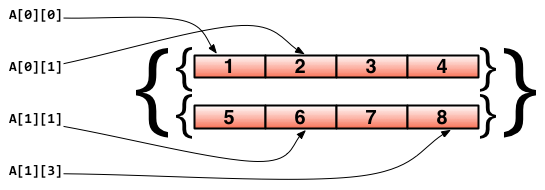
\includegraphics[width=14cm]{2.2.array.png}
   \label{図2.2}
   \caption{多次元配列のマッピング関係}
\end{figure}


\paragraph{slice}
多くのアプリケーションでは、配列はあまりわたしたちの要求を満たしてはくれません。配列を初期化する場合、どれぐらいの大きさの配列が必要かわからないからです。そのため、"動的な配列"が必要となります。Goではこのようなデータ構造を\texttt{slice}と呼びます。

\texttt{slice}は本当の意味での動的な配列ではありません。これは単なる参照型です。\texttt{slice}は常に低レイヤの\texttt{array}を指しています。\texttt{slice}の宣言も\texttt{array}と同様に長さを指定する必要はありません。

\begin{lstlisting}[numbers=none]
// arrayの宣言と同じですが、長さは必要ありません。
var fslice []int
\end{lstlisting}

次に\texttt{slice}を宣言すると同時にデータを初期化します:

\begin{lstlisting}[numbers=none]
slice := []byte {'a', 'b', 'c', 'd'}
\end{lstlisting}

\texttt{slice}はひとつの配列またはすでに存在する\texttt{slice}の中から宣言することができます。\texttt{slice}は\texttt{array[i:j]}で取得することができます。この中で\texttt{i}は配列の開始位置です。\texttt{j}は終了位置です。ただし\texttt{array[j]}は含みません。長さは\texttt{j-i}となります。

\begin{lstlisting}[numbers=none]
// 10個の要素を宣言します。要素の型はbyteの配列です。
var ar = [10]byte {'a', 'b', 'c', 'd', 'e',
                   'f', 'g', 'h', 'i', 'j'}

// byteを含む2つのsliceを宣言します
var a, b []byte

    // aポインタ配列の3つ目の要素から始まり、5つ目の要素まで
a = ar[2:5]
    //現在aの持つ要素は:ar[2]、ar[3]とar[4]です。

    // bは配列arのもう一つのsliceです。
b = ar[3:5]
// bの要素は:ar[3]とar[4]です。
\end{lstlisting}

\begin{quote}
  \texttt{slice}と配列は宣言時に区別されますのでご注意ください:配列を宣言するとき、中括弧の中で配列の長さを明示するかまたは\texttt{...}で自動的に長さを計算します。一方\texttt{slice}を宣言する時は、中括弧内には文字はありません。
\end{quote}

これらのデータ構造は以下のようになっています。

\begin{figure}[H]
  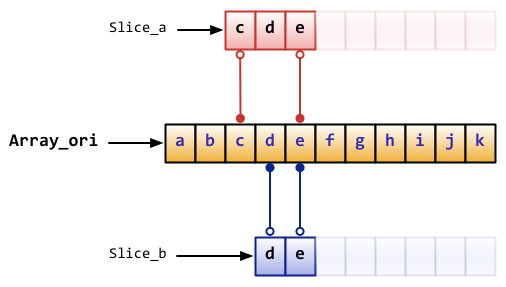
\includegraphics[width=14cm]{2.2.slice.png}
   \label{図2.3}
   \caption{sliceとarrayの対応関係図}
\end{figure}

sliceには便利な操作があります

\begin{itemize}
  \item \texttt{slice}のデフォルト開始位置は0です。\texttt{ar[:n]}などは\texttt{ar[0:n]}と等価です。
  \item \texttt{slice}の2つ目の値のデフォルトは配列の長さです。\texttt{ar[n:]}は\texttt{ar[n:len(ar)]}等価です。
  \item もし配列の中から直接\texttt{slice}を取り出す場合は、\texttt{ar[:]}というような形で指定することができます。なぜならデフォルトのはじめの値は0で2つ目は配列の長さだからです。すなわち、\texttt{ar[0:len(ar)]}と等価となります。
\end{itemize}

ここではより多くの\texttt{slice}の操作についていくつか例を挙げます:

\begin{lstlisting}[numbers=none]
// 配列を宣言
var array = [10]byte{'a', 'b', 'c', 'd', 'e',
                     'f', 'g', 'h', 'i', 'j'}
// sliceを2つ宣言
var aSlice, bSlice []byte

// 便利な操作のデモンストレーション
aSlice = array[:3] // aSlice = array[0:3] と同じ。
// aSliceには以下の要素が含まれます: a,b,c
aSlice = array[5:] // aSlice = array[5:10] と同じ。
// aSliceには以下の要素が含まれます: f,g,h,i,j
aSlice = array[:]  // aSlice = array[0:10] と同じ。
// この場合aSliceにはすべての要素が含まれます。

// sliceからsliceを取り出す
aSlice = array[3:7]  // aSliceには以下の要素が含まれます:
                     // d,e,f,g,len=4,cap=7
bSlice = aSlice[1:3] // bSlice にはaSlice[1], aSlice[2] が
// 含まれそれぞれの要素は以下のとおりです: e,f
bSlice = aSlice[:3]  // bSlice には aSlice[0], aSlice[1],
// aSlice[2] が含まれます。それぞれ以下のとおりです: d,e,f
bSlice = aSlice[0:5] // sliceのsliceに対してcapの
// 範囲内で拡張することができます。
// この時bSliceには以下の要素が含まれます:d,e,f,g,h
bSlice = aSlice[:]   // bSliceにはaSliceのすべての
                     // 要素が含まれます: d,e,f,g
\end{lstlisting}

\texttt{slice}は参照型ですので、この中の要素の値を変更すると、そのほかのすべての参照でも値が変更されます。たとえば上の\texttt{aSlice}と\texttt{bSlice}で、\texttt{aSlice}の中の要素を変更すると、\texttt{bSlice}の対応する値も同時に変更されます。

概念上では、\texttt{slice}は構造体です。この構造体には3つの要素が含まれます: 

\begin{itemize}
  \item 一つはポインタです。配列中の\texttt{slice}が示す開始位置を指しています。
  \item 長さ、つまり\texttt{slice}の長さです。
  \item 最大の長さ、\texttt{slice}の開始位置から配列の最後の位置までの長さです。
\end{itemize}


\begin{lstlisting}[numbers=none]
Array_a := [10]byte{'a', 'b', 'c', 'd', 'e', 'f', 'g', 'h', 'i', 'j'}
Slice_a := Array_a[2:5]
\end{lstlisting}

上のコードの正しい保存構造は下の図に示す通りです。

\begin{figure}[H]
  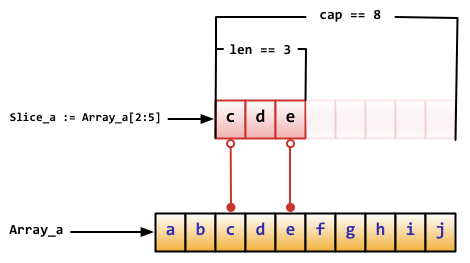
\includegraphics[width=14cm]{2.2.slice2.png}
   \label{図2.4}
   \caption{sliceに対応する配列の情報}
\end{figure}

\texttt{slice}に対しては、いくつかの便利なビルトイン関数があります:

\begin{description}
  \item[\texttt{len}] \texttt{slice}の長さを取得します。
  \item[\texttt{cap}] \texttt{slice}の最大容量を取得します。
  \item[\texttt{append}] \texttt{slice}に対して一つまたは複数の要素を追加します。その後\texttt{slice}と同じ型の\texttt{slice}を返します。
  \item[\texttt{copy}] 関数\texttt{copy}はもとの\texttt{slice}の\texttt{src}を\texttt{dst}に要素をコピーし、コピーした要素の個数を返します。
\end{description}

注:\texttt{append}関数は\texttt{slice}が参照した配列の内容を変更し得ます。そのため、参照先と同一の配列の他の\texttt{slice}にも影響します。 しかし\texttt{slice}の中に余分なスペースが無い(\texttt{(cap-len) == 0})場合、動的なメモリから新たな配列空間が割り当てられます。返される\texttt{slice}配列のポインタはこの空間を指しています。また、もとの配列の内容は変わりません。この配列を参照している他の\texttt{slice}は影響を受けません。

Go1.2より、sliceは三引数のsliceをサポートするようになりました。以前まで我々は以下のような方法でsliceまたはarrayからsliceを取り出していました

\begin{lstlisting}[numbers=none]
var array [10]int
slice := array[2:4]
\end{lstlisting}

この例ではsliceの要素数は8で、新しいバージョンでは以下のように要素数を指定することができます

\begin{lstlisting}[numbers=none]
slice = array[2:4:7]
\end{lstlisting}

上の要素数は\texttt{7-2}、即ち\texttt{5}となります。このように生成された新しいsliceでは最後の3つの要素にアクセスする方法がなくなります。

もしsliceが\texttt{array[:i:j]}のような形式だった場合は、第一引数は空と見なされ、デフォルトの0となります。



\paragraph{map}
\texttt{map}の概念もPythonのディクショナリです。この形式は\texttt{map[keyType]valueType}です。

下のコードをご覧ください。\texttt{map}の読み込みと代入は\texttt{slice}と似ています。\texttt{key}を通して操作します。ただ、\texttt{slice}の\texttt{index}は\texttt{int}型のみになります。\texttt{map}には多くの型があります。\texttt{int}でもかまいませんし、\texttt{string}や\texttt{==}と\texttt{!=}演算子が定義されている全ての型でもかまいません。

\begin{lstlisting}[numbers=none]
  // keyを文字列で宣言します。値はintとなるディクショナリです。
  // この方法は使用される前にmakeで初期化される必要があります。
var numbers map[string]int
// もうひとつのmapの宣言方法
numbers := make(map[string]int)
numbers["one"] = 1  //代入
numbers["ten"] = 10 //代入
numbers["three"] = 3

fmt.Println("3つ目の数字は: ", numbers["three"]) // データの取得
// "3つ目の数字は: 3"という風に出力されます。
\end{lstlisting}

この\texttt{map}は我々が普段目にする表と同じです。左の列に\texttt{key}、右の列に値があります。

mapを使う段階で注意しなければならないことがいくつかあります:

\begin{itemize}
\item \texttt{map}は順序がありません。毎回\texttt{map}の出力は違ったものになるかもしれません。\texttt{index}で値を取得することはできず、かならず\texttt{key}を使うことになります。
\item \texttt{map}の長さは固定ではありません。\texttt{slice}と同じで、参照型の一種です。
\item ビルトインの\texttt{len}関数を\texttt{map}に適用すると、\texttt{map}がもつ\texttt{key}の個数を返します。
\item \texttt{map}の値は簡単に修正することができます。\texttt{numbers["one"]=11}というようにkeyが\texttt{one}のディクショナリの値を\texttt{11}に変えることができます。
\item \texttt{map}は他の基本型と異なり、thread-safeではありません。複数のgo-routineを扱う際には必ずmutex lockメカニズムを使用する必要があります。
\end{itemize}

\texttt{map}の初期化では\texttt{key:val}の方法で初期値を与えることができます。また同時に\texttt{map}には標準で\texttt{key}が存在するか確認する方法が存在します。

\texttt{delete}で\texttt{map}の要素を削除します:

\begin{lstlisting}[numbers=none]
// ディクショナリを初期化します。
rating := map[string]float32{"C":5, "Go":4.5,
                             "Python":4.5, "C++":2 }
// mapは2つの戻り値があります。2つ目の戻り値では、
// もしkeyが存在しなければ、okはfalseに、存在すれ
// ばokはtrueになります。
csharpRating, ok := rating["C#"]
if ok {
fmt.Println("C# is in the map and its rating is ",
            csharpRating)
} else {
fmt.Println("We have no rating associated
             with C# in the map")
}

delete(rating, "C")  // keyがCの要素を削除します。
\end{lstlisting}

上述の通り、\texttt{map}は参照型の一種ですので、もし2つの\texttt{map}が同時に同じポインタを指している場合、一つの変更で、もう一つにも変更が行われます。

\begin{lstlisting}[numbers=none]
m := make(map[string]string)
m["Hello"] = "Bonjour"
m1 := m
m1["Hello"] = "Salut" // この時、m["hello"]の
                // 値もすでにSalutになっています。
\end{lstlisting}





\paragraph{make, new操作}
\texttt{make}はビルトイン型(\texttt{map}、\texttt{slice}および\texttt{channel})のメモリの割り当てです。\texttt{new}は各型のメモリを割り当てます。

ビルトイン関数\texttt{new}は本質的には他の言語で使われる同名の関数と機能が同じです:\texttt{new(T)}はゼロサプレスされた\texttt{T}型のメモリ空間を割り当て、そのアドレスを返します。すなわち\texttt{*T}型の値です。Goの専門用語で言えば、ポインタを返すということです。新たに割り当てられた型\texttt{T}のゼロ値です。とても重要なことに:

\begin{quote}
\texttt{new}はポインタを返します。
\end{quote}

ビルトイン関数\texttt{make(T, args)}と\texttt{new(T)}は異なる機能を持っています。makeは\texttt{slice}、\texttt{map}または\texttt{channel}を作成し、初期値(非ゼロ値)を持つ\texttt{T}型を返すのみで、\texttt{*T}ではありません。本質的には、この3つの型が異なる点はデータ構造を指し示す参照が使用される前に初期化されているということです。例えば、データ(内部\texttt{array})を指し示すポインタ、長さ,容量による3点で記述される\texttt{slice}の各項目が初期化される前は、\texttt{slice}は\texttt{nil}です。\texttt{slice}, \texttt{map}, \texttt{channel}にとって、makeは内部のデータ構造を初期化し、適当な値で埋め尽くされます。


\begin{quote}
\texttt{make}は初期化後の(非ゼロの)値を返します。
\end{quote}




\begin{figure}[H]
  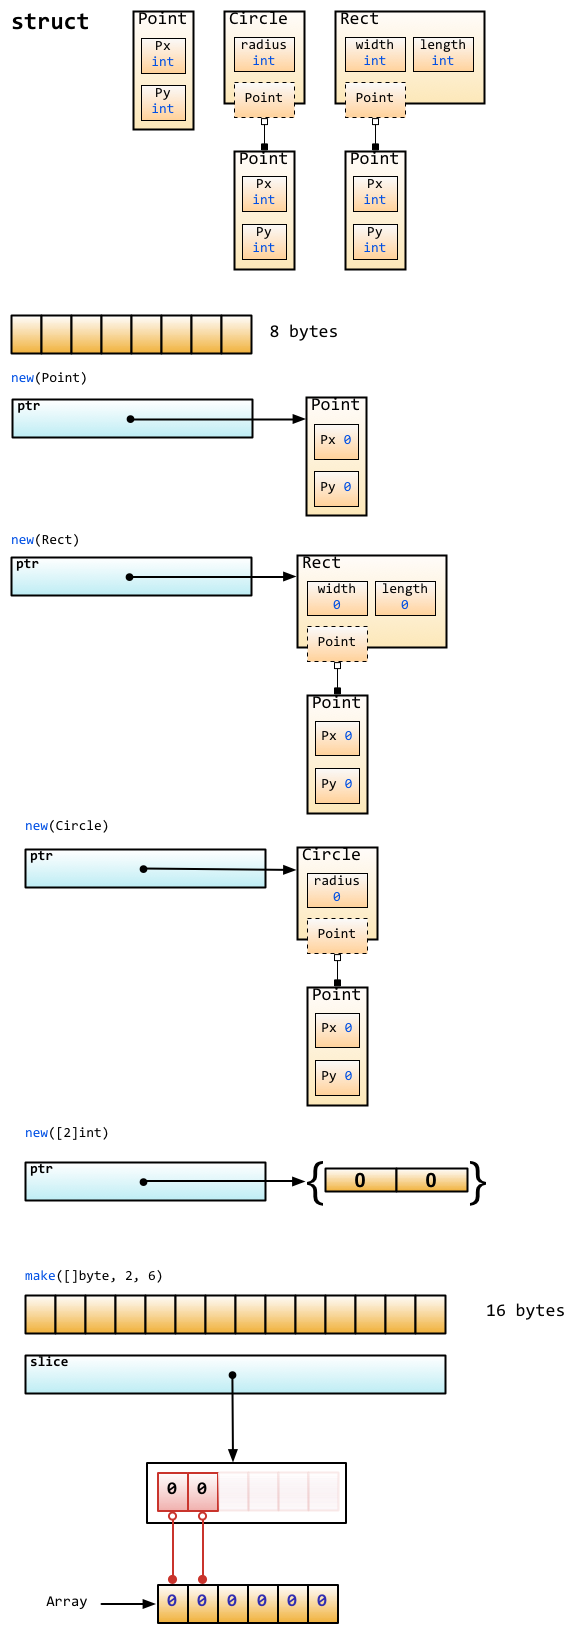
\includegraphics[width=7cm]{2.2.makenew.png}
   \label{図2.5}
   \caption{makeとnewの低レイヤでのメモリの割り当て}
\end{figure}

\subsubsection{ゼロ値}
"ゼロ値"というのは何も空の値ではありません。これは一種の"変数が埋めらる前"のデフォルト値であり、通常は0です。 それぞれの型のゼロ値は以下の通りです


\begin{lstlisting}[numbers=none]
int     0
int8    0
int32   0
int64   0
uint    0x0
rune    0 //runeの実際の型は int32 です。
byte    0x0 // byteの実際の型は uint8 です。
float32 0 //長さは 4 byte
float64 0 //長さは 8 byte
bool    false
string  ""
\end{lstlisting}

